\documentclass[10pt]{article}
\usepackage[polish]{babel}
\usepackage[utf8]{inputenc}
\usepackage[T1]{fontenc}
\usepackage{graphicx}
\usepackage[export]{adjustbox}
\graphicspath{ {./images/} }
\usepackage{amsmath}
\usepackage{amsfonts}
\usepackage{amssymb}
\usepackage[version=4]{mhchem}
\usepackage{stmaryrd}
\usepackage{multirow}
\usepackage{hyperref}
\hypersetup{colorlinks=true, linkcolor=blue, filecolor=magenta, urlcolor=cyan,}
\urlstyle{same}

\title{KOD }

\author{}
\date{}


\begin{document}
\maketitle
IMIĘ I NAZWISKO *\\
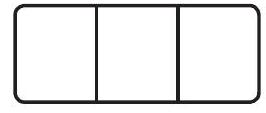
\includegraphics[max width=\textwidth, center]{2024_11_21_5229b9d0453456f1828dg-01}\\
\(\square\)

\begin{itemize}
  \item nieobowiązkowe
\end{itemize}

\section*{PRÓBNY EGZAMIN MATURALNY Z NOWĄ ERĄ MATEMATYKA - POZIOM ROZSZERZONY}
\section*{Instrukcja dla zdającego}
\begin{enumerate}
  \item Sprawdź, czy arkusz egzaminacyjny zawiera 22 strony (zadania 1-17). Ewentualny brak stron zgłoś nauczycielowi nadzorującemu egzamin.
  \item Rozwiązania zadań i odpowiedzi zapisz w miejscu na to przeznaczonym.
  \item Pamiętaj, że pominięcie argumentacji lub istotnych obliczeń w rozwiązaniu zadań otwartych może spowodować, że za to rozwiązanie nie otrzymasz pełnej liczby punktów.
  \item Pisz czytelnie. Używaj długopisu/pióra tylko z czarnym tuszem/atramentem.
  \item Nie używaj korektora, a błędne zapisy wyraźnie przekreśl.
  \item Pamiętaj, że zapisy w brudnopisie nie będą oceniane.
  \item Podczas egzaminu możesz korzystać z zestawu wzorów matematycznych, cyrkla i linijki oraz kalkulatora prostego.
  \item Na tej stronie wpisz swój kod oraz imię i nazwisko.
  \item Nie wpisuj żadnych znaków w części przeznaczonej dla osoby sprawdzającej.\\
\(\square\) dysleksja
\end{enumerate}

STYCZEŃ 2017

Czas pracy:\\
180 minut

Liczba punktów\\
do uzyskania: 50

W zadaniach 1.-5. wybierz i zaznacz poprawną odpowiedź.

\section*{Zadanie 1. (0-1)}
Dane są liczby \(a=\log _{3} 5, \quad b=\log _{5} 7, \quad c=\log _{7} 3\). Iloczyn \(a b c\) jest równy\\
A. 1\\
B. 3\\
C. 5\\
D. 7

Zadanie 2. (0-1)\\
Ciąg \(\left(a_{n}\right)\) jest określony następująco: \(a_{1}=\left(\frac{3}{2}\right)^{100}\) oraz \(a_{n+1}=\left(\frac{2}{3}\right) \cdot a_{n}\) dla \(n \geqslant 1\). Wówczas\\
A. \(a_{99}=1\)\\
B. \(a_{100}=1\)\\
C. \(a_{101}=1\)\\
D. \(a_{102}=1\)

\section*{Zadanie 3. (0-1)}
Równanie \(x^{5}+x^{3}+x=0\)\\
A. nie ma rozwiązań rzeczywistych.\\
B. ma dokładnie jedno rozwiązanie rzeczywiste.\\
C. ma dokładnie trzy rozwiązania rzeczywiste.\\
D. ma dokładnie pięć rozwiązań rzeczywistych.

\section*{Zadanie 4. (0-1)}
Wartość wyrażenia \(2 \cos ^{2} 15^{\circ}-1\) jest równa\\
A. \(-\frac{\sqrt{3}}{2}\)\\
B. \(-\frac{1}{2}\)\\
C. \(\frac{\sqrt{2}}{2}\)\\
D. \(\frac{\sqrt{3}}{2}\)

\section*{Zadanie 5. (0-1)}
Okrąg o środku \(S=(-1,2)\) jest styczny do prostej o równaniu \(3 x+4 y+5=0\). Promień tego okręgu jest równy\\
A. 1\\
B. 2\\
C. 4\\
D. 16

\section*{BRUDNOPIS}
\begin{center}
\begin{tabular}{|c|c|c|c|c|c|c|c|c|c|c|c|c|c|c|c|c|c|c|c|c|c|c|c|c|c|c|c|c|c|}
\hline
 &  &  &  &  &  &  &  &  &  &  &  &  &  &  &  &  &  &  &  &  &  &  &  &  &  &  &  &  &  \\
\hline
 &  &  &  &  &  &  &  &  &  &  &  &  &  &  &  &  &  &  &  &  &  &  &  &  &  &  &  &  &  \\
\hline
 &  &  &  &  &  &  &  &  &  &  &  &  &  &  &  &  &  &  &  &  &  &  &  &  &  &  &  &  &  \\
\hline
 &  &  &  &  &  &  &  &  &  &  &  &  &  &  &  &  &  &  &  &  &  &  &  &  &  &  &  &  &  \\
\hline
 &  &  &  &  &  &  &  &  &  &  &  &  &  &  &  &  &  &  &  &  &  &  &  &  &  &  &  &  &  \\
\hline
 &  &  &  &  &  &  &  &  &  &  &  &  &  &  &  &  &  &  &  &  &  &  &  &  &  &  &  &  &  \\
\hline
 &  &  &  &  &  &  &  &  &  &  &  &  &  &  &  &  &  &  &  &  &  &  &  &  &  &  &  &  &  \\
\hline
 &  &  &  &  &  &  &  &  &  &  &  &  &  &  &  &  &  &  &  &  &  &  &  &  &  &  &  &  &  \\
\hline
 &  &  &  &  &  &  &  &  &  &  &  &  &  &  &  &  &  &  &  &  &  &  &  &  &  &  &  &  &  \\
\hline
 &  &  &  &  &  &  &  &  &  &  &  &  &  &  &  &  &  &  &  &  &  &  &  &  &  &  &  &  &  \\
\hline
 &  &  &  &  &  &  &  &  &  &  &  &  &  &  &  &  &  &  &  &  &  &  &  &  &  &  &  &  &  \\
\hline
\end{tabular}
\end{center}

\begin{center}

\includegraphics[max width=\textwidth]{2024_11_21_5229b9d0453456f1828dg-03}
\end{center}

\begin{center}
\begin{tabular}{|c|l|c|c|c|c|c|}
\hline
\multirow{2}{*}{\begin{tabular}{c}
Wypełnia \\
sprawdzający \\
\end{tabular}} & Nr zadania & 1 & 2 & 3 & 4 & 5 \\
\cline { 2 - 7 }
 & Maks. liczba pkt & 1 & 1 & 1 & 1 & 1 \\
\cline { 2 - 7 }
 & Uzyskana liczba pkt &  &  &  &  &  \\
\hline
\end{tabular}
\end{center}

W zadaniu 6. zakoduj wynik w kratkach zamieszczonych pod poleceniem.\\
\(W\) zadaniach 7.-17. rozwiązania zapisz w wyznaczonych miejscach pod treścia zadania.

\section*{Zadanie 6. (0-2)}
Liczby \(a\) i \(b\) spełniają warunki \(a+b=6\) i \(a \cdot b=2\). Oblicz wartość wyrażenia \(a^{3}+b^{3}\).\\
Wpisz w poniższe kratki kolejno: cyfrę setek, cyfrę dziesiątek i cyfrę jedności otrzymanego wyniku.\\
\(\square\)

Więcej arkuszy znajdziesz na stronie: \href{http://arkusze.pl}{arkusze.pl}\\

\includegraphics[max width=\textwidth, center]{2024_11_21_5229b9d0453456f1828dg-04}

Zadanie 7. (0-2)\\
Oblicz \(\lim _{n \rightarrow \infty} \frac{(n-1)^{2}}{(2 n-2)^{2}+(6 n+3)^{2}}\).\\

\includegraphics[max width=\textwidth, center]{2024_11_21_5229b9d0453456f1828dg-05}

Odpowiedź:

\begin{center}
\begin{tabular}{|l|l|c|c|}
\hline
\multirow{2}{*}{\begin{tabular}{c}
Wypełnia \\
sprawdzający \\
\end{tabular}} & Nr zadania & 6 & 7 \\
\cline { 2 - 4 }
 & Maks. liczba pkt & 2 & 2 \\
\cline { 2 - 4 }
 & Uzyskana liczba pkt &  &  \\
\hline
\end{tabular}
\end{center}

Zadanie 8. (0-2)\\
Dana jest funkcja kwadratowa \(f(x)=x^{2}-120\). Oblicz największą wartość funkcji kwadratowej \(g\) określonej wzorem \(g(x)=-2 \cdot f(x+4)-6\).\\

\includegraphics[max width=\textwidth, center]{2024_11_21_5229b9d0453456f1828dg-06}

Odpowiedź:

Zadanie 9. (0-2)\\
W nieskończonym ciągu geometrycznym \(\left(a_{n}\right)\) dane są: \(a_{1}=k, a_{2}=k-1\), gdzie \(k>1\).\\
Suma wszystkich wyrazów tego ciągu jest równa 5 . Oblicz \(k\).\\

\includegraphics[max width=\textwidth, center]{2024_11_21_5229b9d0453456f1828dg-07}

Odpowiedź:

\begin{center}
\begin{tabular}{|l|l|c|c|}
\hline
\multirow{2}{*}{\begin{tabular}{c}
Wypełnia \\
sprawdzający \\
\end{tabular}} & Nr zadania & 8 & 9 \\
\cline { 2 - 4 }
 & Maks. liczba pkt & 2 & 2 \\
\cline { 2 - 4 }
 & Uzyskana liczba pkt &  &  \\
\hline
\end{tabular}
\end{center}

Zadanie 10. (0-4)\\
Rozwiąż równanie \(2 \cos 2 x \cos 5 x=\cos 7 x+\frac{1}{2} \mathrm{w}\) przedziale \(\langle 0, \pi\rangle\).

Więcej arkuszy znajdziesz na stronie: \href{http://arkusze.pl}{arkusze.pl}\\

\includegraphics[max width=\textwidth, center]{2024_11_21_5229b9d0453456f1828dg-08}\\

\includegraphics[max width=\textwidth, center]{2024_11_21_5229b9d0453456f1828dg-09}

Odpowiedź:

\begin{center}
\begin{tabular}{|l|l|c|}
\hline
\multirow{2}{*}{\begin{tabular}{c}
Wypełnia \\
sprawdzający \\
\end{tabular}} & Nr zadania & 10 \\
\cline { 2 - 3 }
 & Maks. liczba pkt & 4 \\
\cline { 2 - 3 }
 & Uzyskana liczba pkt &  \\
\hline
\end{tabular}
\end{center}

\section*{Zadanie 11. (0-4)}
Wyznacz wszystkie wartości parametru \(m\), dla których funkcja kwadratowa

\[
f(x)=x^{2}-(4 m+2) x+4 m^{2}+4 m-3
\]

ma dwa różne miejsca zerowe \(x_{1}\) i \(x_{2}\) spełniające warunek \(x_{1}+x_{2}=\left|x_{1}-x_{2}\right|\).\\

\includegraphics[max width=\textwidth, center]{2024_11_21_5229b9d0453456f1828dg-10}\\

\includegraphics[max width=\textwidth, center]{2024_11_21_5229b9d0453456f1828dg-11}

Odpowiedź:

\begin{center}
\begin{tabular}{|l|l|c|}
\hline
\multirow{2}{*}{\begin{tabular}{c}
Wypełnia \\
sprawdzający \\
\end{tabular}} & Nr zadania & 11 \\
\cline { 2 - 3 }
 & Maks. liczba pkt & 4 \\
\cline { 2 - 3 }
 & Uzyskana liczba pkt &  \\
\hline
\end{tabular}
\end{center}

Zadanie 12. (0-3)\\
Udowodnij, że dla dowolnych liczb rzeczywistych \(x, y \mathrm{i} z\) prawdziwa jest nierówność:

\[
3 x^{2}+3 y^{2}+3 z^{2}+4 x y+4 x z+4 y z \geqslant 0
\]


\includegraphics[max width=\textwidth, center]{2024_11_21_5229b9d0453456f1828dg-12(3)}\\
\(\qquad\)\\
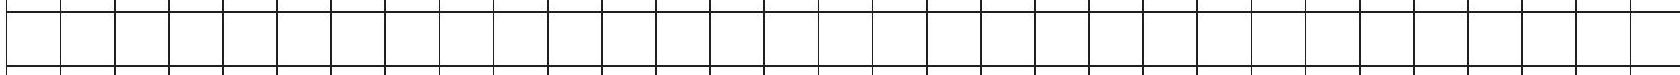
\includegraphics[max width=\textwidth, center]{2024_11_21_5229b9d0453456f1828dg-12(1)}\\
\(\qquad\)\\
\(\qquad\)\\
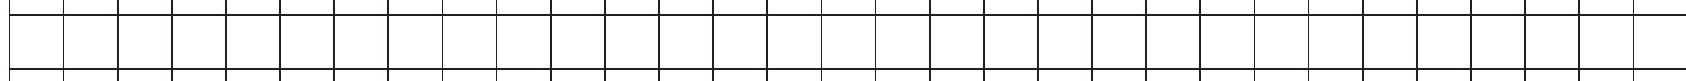
\includegraphics[max width=\textwidth, center]{2024_11_21_5229b9d0453456f1828dg-12}\\

\includegraphics[max width=\textwidth, center]{2024_11_21_5229b9d0453456f1828dg-12(2)}

Zadanie 13. (0-4)\\
Rzucamy trzema symetrycznymi sześciennymi kostkami do gry. Oblicz prawdopodobieństwo warunkowe \(P(A \mid B)\), gdzie \(A\) to zdarzenie polegające na tym, że suma wyrzuconych oczek na wszystkich kostkach będzie parzysta, a \(B\) to zdarzenie, w którym dokładnie na jednej kostce wypadnie 6 oczek.\\

\includegraphics[max width=\textwidth, center]{2024_11_21_5229b9d0453456f1828dg-13}

Odpowiedź:

\begin{center}
\begin{tabular}{|l|l|c|c|}
\hline
\multirow{2}{*}{\begin{tabular}{c}
Wypełnia \\
sprawdzający \\
\end{tabular}} & Nr zadania & 12 & 13 \\
\cline { 2 - 4 }
 & Maks. liczba pkt & 3 & 4 \\
\cline { 2 - 4 }
 & Uzyskana liczba pkt &  &  \\
\hline
\end{tabular}
\end{center}

Zadanie 14. (0-4)\\
Czworokąt \(A B C D\) o bokach długości \(|A B|=24,|B C|=20,|C D|=15\) i \(|A D|=7\) wpisano w okrąg. Oblicz długość przekątnej \(A C\) tego czworokąta.\\

\includegraphics[max width=\textwidth, center]{2024_11_21_5229b9d0453456f1828dg-14}

\begin{center}
\begin{tabular}{|c|c|c|c|c|c|c|c|c|c|c|c|c|c|c|c|c|c|c|c|c|c|c|c|c|c|c|c|c|c|c|}
\hline
 &  &  &  &  &  &  &  &  &  &  &  &  &  &  &  &  &  &  &  &  &  &  &  &  &  &  &  &  &  &  \\
\hline
 &  &  &  &  &  &  &  &  &  &  &  &  &  &  &  &  &  &  &  &  &  &  &  &  &  &  &  &  &  &  \\
\hline
 &  &  &  &  &  &  &  &  &  &  &  &  &  &  &  &  &  &  &  &  &  &  &  &  &  &  &  &  &  &  \\
\hline
 &  &  &  &  &  &  &  &  &  &  &  &  &  &  &  &  &  &  &  &  &  &  &  &  &  &  &  &  &  &  \\
\hline
 &  &  &  &  &  &  &  &  &  &  &  &  &  &  &  &  &  &  &  &  &  &  &  &  &  &  &  &  &  &  \\
\hline
 &  &  &  &  &  &  &  &  &  &  &  &  &  &  &  &  &  &  &  &  &  &  &  &  &  &  &  &  &  &  \\
\hline
 &  &  &  &  &  &  &  &  &  &  &  &  &  &  &  &  &  &  &  &  &  &  &  &  &  &  &  &  &  &  \\
\hline
 &  &  &  &  &  &  &  &  &  &  &  &  &  &  &  &  &  &  &  &  &  &  &  &  &  &  &  &  &  &  \\
\hline
 &  &  &  &  &  &  &  &  &  &  &  &  &  &  &  &  &  &  &  &  &  &  &  &  &  &  &  &  &  &  \\
\hline
 &  &  &  &  &  &  &  &  &  &  &  &  &  &  &  &  &  &  &  &  &  &  &  &  &  &  &  &  &  &  \\
\hline
 &  &  &  &  &  &  &  &  &  &  &  &  &  &  &  &  &  &  &  &  &  &  &  &  &  &  &  &  &  &  \\
\hline
 &  &  &  &  &  &  &  &  &  &  &  &  &  &  &  &  &  &  &  &  &  &  &  &  &  &  &  &  &  &  \\
\hline
 &  &  &  &  &  &  &  &  &  &  &  &  &  &  &  &  &  &  &  &  &  &  &  &  &  &  &  &  &  &  \\
\hline
 &  &  &  &  &  &  &  &  &  &  &  &  &  &  &  &  &  &  &  &  &  &  &  &  &  &  &  &  &  &  \\
\hline
 &  &  &  &  &  &  &  &  &  &  &  &  &  &  &  &  &  &  &  &  &  &  &  &  &  &  &  &  &  &  \\
\hline
 &  &  &  &  &  &  &  &  &  &  &  &  &  &  &  &  &  &  &  &  &  &  &  &  &  &  &  &  &  &  \\
\hline
 &  &  &  &  &  &  &  &  &  &  &  &  &  &  &  &  &  &  &  &  &  &  &  &  &  &  &  &  &  &  \\
\hline
 &  &  &  &  &  &  &  &  &  &  &  &  &  &  &  &  &  &  &  &  &  &  &  &  &  &  &  &  &  &  \\
\hline
 &  &  &  &  &  &  &  &  &  &  &  &  &  &  &  &  &  &  &  &  &  &  &  &  &  &  &  &  &  &  \\
\hline
 &  &  &  &  &  &  &  &  &  &  &  &  &  &  &  &  &  &  &  &  &  &  &  &  &  &  &  &  &  &  \\
\hline
 &  &  &  &  &  &  &  &  &  &  &  &  &  &  &  &  &  &  &  &  &  &  &  &  &  &  &  &  &  &  \\
\hline
 &  &  &  &  &  &  &  &  &  &  &  &  &  &  &  &  &  &  &  &  &  &  &  &  &  &  &  &  &  &  \\
\hline
 &  &  &  &  &  &  &  &  &  &  &  &  &  &  &  &  &  &  &  &  &  &  &  &  &  &  &  &  &  &  \\
\hline
 &  &  &  &  &  &  &  &  &  &  &  &  &  &  &  &  &  &  &  &  &  &  &  &  &  &  &  &  &  &  \\
\hline
 &  &  &  &  &  &  &  &  &  &  &  &  &  &  &  &  &  &  &  &  &  &  &  &  &  &  &  &  &  &  \\
\hline
 &  &  &  &  &  &  &  &  &  &  &  &  &  &  &  &  &  &  &  &  &  &  &  &  &  &  &  &  &  &  \\
\hline
 &  &  &  &  &  &  &  &  &  &  &  &  &  &  &  &  &  &  &  &  &  &  &  &  &  &  &  &  &  &  \\
\hline
 &  &  &  &  &  &  &  &  & 
\includegraphics[max width=\textwidth]{2024_11_21_5229b9d0453456f1828dg-15(1)}
 &  &  &  & \(\square\) & 
\includegraphics[max width=\textwidth]{2024_11_21_5229b9d0453456f1828dg-15(48)}
 & | & . & 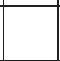
\includegraphics[max width=\textwidth]{2024_11_21_5229b9d0453456f1828dg-15(47)}
 & 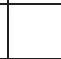
\includegraphics[max width=\textwidth]{2024_11_21_5229b9d0453456f1828dg-15(42)}
 & 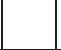
\includegraphics[max width=\textwidth]{2024_11_21_5229b9d0453456f1828dg-15(24)}
 & 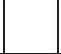
\includegraphics[max width=\textwidth]{2024_11_21_5229b9d0453456f1828dg-15(30)}
 & 
\includegraphics[max width=\textwidth]{2024_11_21_5229b9d0453456f1828dg-15(40)}
 & 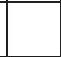
\includegraphics[max width=\textwidth]{2024_11_21_5229b9d0453456f1828dg-15(11)}
 & 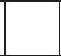
\includegraphics[max width=\textwidth]{2024_11_21_5229b9d0453456f1828dg-15(7)}
 &  &  & 
\includegraphics[max width=\textwidth]{2024_11_21_5229b9d0453456f1828dg-15(39)}
 & 
\includegraphics[max width=\textwidth]{2024_11_21_5229b9d0453456f1828dg-15(32)}
 &  &  &  \\
\hline
 &  &  &  &  &  &  & 
\includegraphics[max width=\textwidth]{2024_11_21_5229b9d0453456f1828dg-15(14)}
 & 
\includegraphics[max width=\textwidth]{2024_11_21_5229b9d0453456f1828dg-15(34)}
 &  & 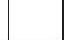
\includegraphics[max width=\textwidth]{2024_11_21_5229b9d0453456f1828dg-15(66)}
 & 
\includegraphics[max width=\textwidth]{2024_11_21_5229b9d0453456f1828dg-15(22)}
 & 
\includegraphics[max width=\textwidth]{2024_11_21_5229b9d0453456f1828dg-15(67)}
 & 
\includegraphics[max width=\textwidth]{2024_11_21_5229b9d0453456f1828dg-15(19)}
 & 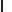
\includegraphics[max width=\textwidth]{2024_11_21_5229b9d0453456f1828dg-15(38)}
 & 
\includegraphics[max width=\textwidth]{2024_11_21_5229b9d0453456f1828dg-15(52)}
 & 
\includegraphics[max width=\textwidth]{2024_11_21_5229b9d0453456f1828dg-15(9)}
 & 
\includegraphics[max width=\textwidth]{2024_11_21_5229b9d0453456f1828dg-15(31)}
 & 
\includegraphics[max width=\textwidth]{2024_11_21_5229b9d0453456f1828dg-15(49)}
 & \(\square\) & 
\includegraphics[max width=\textwidth]{2024_11_21_5229b9d0453456f1828dg-15(4)}
 & - & 
\includegraphics[max width=\textwidth]{2024_11_21_5229b9d0453456f1828dg-15(53)}
 & 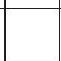
\includegraphics[max width=\textwidth]{2024_11_21_5229b9d0453456f1828dg-15(35)}
 & 
\includegraphics[max width=\textwidth]{2024_11_21_5229b9d0453456f1828dg-15(64)}
 &  & 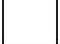
\includegraphics[max width=\textwidth]{2024_11_21_5229b9d0453456f1828dg-15(46)}
 & 
\includegraphics[max width=\textwidth]{2024_11_21_5229b9d0453456f1828dg-15(2)}
 &  &  &  \\
\hline
 &  &  &  &  &  &  &  &  &  & 
\includegraphics[max width=\textwidth]{2024_11_21_5229b9d0453456f1828dg-15(36)}
 & 
\includegraphics[max width=\textwidth]{2024_11_21_5229b9d0453456f1828dg-15(21)}
 & 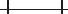
\includegraphics[max width=\textwidth]{2024_11_21_5229b9d0453456f1828dg-15(16)}
 & 
\includegraphics[max width=\textwidth]{2024_11_21_5229b9d0453456f1828dg-15(26)}
 & 
\includegraphics[max width=\textwidth]{2024_11_21_5229b9d0453456f1828dg-15(3)}
 &  &  &  & H & \( \square \) & 
\includegraphics[max width=\textwidth]{2024_11_21_5229b9d0453456f1828dg-15(12)}
 & \includegraphics[max width=\textwidth]{2024_11_21_5229b9d0453456f1828dg-15(62)}
 &  &  &  &  &  & \includegraphics[max width=\textwidth]{2024_11_21_5229b9d0453456f1828dg-15(17)}
 &  &  &  \\
\hline
 &  &  &  &  &  &  &  &  &  &  &  &  &  &  &  &  &  &  &  &  &  &  &  &  &  &  & \includegraphics[max width=\textwidth]{2024_11_21_5229b9d0453456f1828dg-15(18)}
 &  &  &  \\
\hline
 &  &  &  &  &  &  &  &  &  &  &  &  & \includegraphics[max width=\textwidth]{2024_11_21_5229b9d0453456f1828dg-15(73)}
 & \includegraphics[max width=\textwidth]{2024_11_21_5229b9d0453456f1828dg-15(75)}
 &  &  &  & \includegraphics[max width=\textwidth]{2024_11_21_5229b9d0453456f1828dg-15(8)}
 &  &  &  &  &  &  &  &  &  &  &  &  \\
\hline
 &  &  &  &  &  & \includegraphics[max width=\textwidth]{2024_11_21_5229b9d0453456f1828dg-15(50)}
 &  & \includegraphics[max width=\textwidth]{2024_11_21_5229b9d0453456f1828dg-15(6)}
 &  & \includegraphics[max width=\textwidth]{2024_11_21_5229b9d0453456f1828dg-15(5)}
 & \includegraphics[max width=\textwidth]{2024_11_21_5229b9d0453456f1828dg-15(60)}
 & \includegraphics{smile-ee4a42c95f0314155b7fadfb9b76ec05e254f576} & \(\square\) & \includegraphics[max width=\textwidth]{2024_11_21_5229b9d0453456f1828dg-15(29)}
 & \includegraphics[max width=\textwidth]{2024_11_21_5229b9d0453456f1828dg-15(20)}
 & \(\square\) & \includegraphics[max width=\textwidth]{2024_11_21_5229b9d0453456f1828dg-15(65)}
 & \includegraphics[max width=\textwidth]{2024_11_21_5229b9d0453456f1828dg-15}
 & \includegraphics{smile-b35b00a09257720487855e6837f96b3041054db4} & \includegraphics{smile-ddbe84c7690570150a145c497efb8911650a2435} &  & \includegraphics[max width=\textwidth]{2024_11_21_5229b9d0453456f1828dg-15(58)}
 & \includegraphics[max width=\textwidth]{2024_11_21_5229b9d0453456f1828dg-15(27)}
 &  &  & \includegraphics[max width=\textwidth]{2024_11_21_5229b9d0453456f1828dg-15(70)}
 & \includegraphics[max width=\textwidth]{2024_11_21_5229b9d0453456f1828dg-15(10)}
 &  &  &  \\
\hline
 &  &  &  &  &  &  &  &  &  & \includegraphics[max width=\textwidth]{2024_11_21_5229b9d0453456f1828dg-15(61)}
 &  &  & \includegraphics{smile-1ce70be9385ae40d545ccaf9c545a9c3af86f2fa} & \includegraphics[max width=\textwidth]{2024_11_21_5229b9d0453456f1828dg-15(59)}
 &  &  &  & \includegraphics[max width=\textwidth]{2024_11_21_5229b9d0453456f1828dg-15(23)}
 &  & \includegraphics[max width=\textwidth]{2024_11_21_5229b9d0453456f1828dg-15(57)}
 & \includegraphics[max width=\textwidth]{2024_11_21_5229b9d0453456f1828dg-15(74)}
 & \includegraphics[max width=\textwidth]{2024_11_21_5229b9d0453456f1828dg-15(54)}
 &  &  &  &  & \includegraphics[max width=\textwidth]{2024_11_21_5229b9d0453456f1828dg-15(55)}
 &  &  &  \\
\hline
 &  &  &  &  &  &  &  &  &  &  &  &  & \includegraphics{smile-b2d9a146469960129be95b0d548548bcb9c731b2} &  &  &  &  & \includegraphics[max width=\textwidth]{2024_11_21_5229b9d0453456f1828dg-15(56)}
 &  &  &  & \includegraphics[max width=\textwidth]{2024_11_21_5229b9d0453456f1828dg-15(68)}
 &  &  &  &  & \includegraphics[max width=\textwidth]{2024_11_21_5229b9d0453456f1828dg-15(25)}
 &  &  &  \\
\hline
 &  &  &  &  &  &  &  &  &  &  &  &  &  & \includegraphics[max width=\textwidth]{2024_11_21_5229b9d0453456f1828dg-15(43)}
 &  &  &  & \includegraphics[max width=\textwidth]{2024_11_21_5229b9d0453456f1828dg-15(72)}
 & \includegraphics[max width=\textwidth]{2024_11_21_5229b9d0453456f1828dg-15(45)}
 & \includegraphics[max width=\textwidth]{2024_11_21_5229b9d0453456f1828dg-15(33)}
 &  & \includegraphics[max width=\textwidth]{2024_11_21_5229b9d0453456f1828dg-15(63)}
 & \includegraphics[max width=\textwidth]{2024_11_21_5229b9d0453456f1828dg-15(71)}
 &  &  &  & \includegraphics[max width=\textwidth]{2024_11_21_5229b9d0453456f1828dg-15(76)}
 &  &  &  \\
\hline
 &  &  &  &  &  &  &  &  &  & \includegraphics[max width=\textwidth]{2024_11_21_5229b9d0453456f1828dg-15(69)}
 & \includegraphics[max width=\textwidth]{2024_11_21_5229b9d0453456f1828dg-15(37)}
 & \includegraphics[max width=\textwidth]{2024_11_21_5229b9d0453456f1828dg-15(41)}
 &  &  & \includegraphics[max width=\textwidth]{2024_11_21_5229b9d0453456f1828dg-15(51)}
 & \includegraphics[max width=\textwidth]{2024_11_21_5229b9d0453456f1828dg-15(13)}
 & \( 2 \) & \includegraphics[max width=\textwidth]{2024_11_21_5229b9d0453456f1828dg-15(44)}
 & \includegraphics[max width=\textwidth]{2024_11_21_5229b9d0453456f1828dg-15(28)}
 & \includegraphics[max width=\textwidth]{2024_11_21_5229b9d0453456f1828dg-15(15)}
 &  &  &  &  &  &  &  &  &  &  \\
\hline
 &  &  &  &  &  &  &  &  &  &  &  &  &  &  &  &  &  &  &  &  &  &  &  &  &  &  &  &  &  &  \\
\hline
 &  &  &  &  &  &  &  &  &  &  &  &  &  &  &  &  &  &  &  &  &  &  &  &  &  &  &  &  &  &  \\
\hline
\end{tabular}
\end{center}

Odpowiedź:

\begin{center}
\begin{tabular}{|l|l|c|}
\hline
\multirow{3}{*}{\begin{tabular}{c}
Wypełnia \\
sprawdzający \\
\end{tabular}} & Nr zadania & 14 \\
\cline { 2 - 3 }
 & Maks. liczba pkt & 4 \\
\cline { 2 - 3 }
 & Uzyskana liczba pkt &  \\
\hline
\end{tabular}
\end{center}

Zadanie 15. (0-5)\\
Punkt \(A=(0,0)\) jest wierzchołkiem równoległoboku \(A B C D\). Punkt \(M=(8,1)\) jest środkiem boku \(B C\), a punkt \(N=(10,5)\) - środkiem boku \(C D\) tego równoległoboku. Oblicz współrzędne wierzchołków: \(B, C\) i \(D\).

Więcej arkuszy znajdziesz na stronie: \href{http://arkusze.pl}{arkusze.pl}\\
\includegraphics[max width=\textwidth, center]{2024_11_21_5229b9d0453456f1828dg-16}\\
\includegraphics[max width=\textwidth, center]{2024_11_21_5229b9d0453456f1828dg-17}

Odpowiedź:

\begin{center}
\begin{tabular}{|l|l|c|}
\hline
\multirow{2}{*}{\begin{tabular}{c}
Wypełnia \\
sprawdzający \\
\end{tabular}} & Nr zadania & 15 \\
\cline { 2 - 3 }
 & Maks. liczba pkt & 5 \\
\cline { 2 - 3 }
 & Uzyskana liczba pkt &  \\
\hline
\end{tabular}
\end{center}

Zadanie 16. (0-6)\\
Krawędź sześcianu \(A B C D E F G H\) ma długość 12. Na krawędziach \(A B\) i \(B C\) wybrano takie punkty \(X\) i \(Y\), że \(|B X|=|B Y|=8\). Przekrój tego sześcianu płaszczyzną XYH jest pięciokątem \(H W X Y Z\) (rysunek niżej).\\
\includegraphics[max width=\textwidth, center]{2024_11_21_5229b9d0453456f1828dg-18}

Oblicz obwód tego pięciokąta.

Więcej arkuszy znajdziesz na stronie: \href{http://arkusze.pl}{arkusze.pl}\\
\includegraphics[max width=\textwidth, center]{2024_11_21_5229b9d0453456f1828dg-18(1)}\\
\includegraphics[max width=\textwidth, center]{2024_11_21_5229b9d0453456f1828dg-19}

Odpowiedź:

\begin{center}
\begin{tabular}{|l|l|c|}
\hline
\multirow{3}{*}{\begin{tabular}{c}
Wypełnia \\
sprawdzający \\
\end{tabular}} & Nr zadania & 16 \\
\cline { 2 - 3 }
 & Maks. liczba pkt & 6 \\
\cline { 2 - 3 }
 & Uzyskana liczba pkt &  \\
\hline
\end{tabular}
\end{center}

\section*{Zadanie 17. (0-7)}
Rozpatrujemy wszystkie prostopadłościany spełniające jednocześnie dwa warunki:

\begin{itemize}
  \item suma długości wszystkich krawędzi jest równa 52,
  \item podstawą jest prostokąt o bokach \(x\) i \(x+3\).
\end{itemize}

Zapisz objętość takiego prostopadłościanu jako funkcję zmiennej \(x\). Wyznacz dziedzinę tej funkcji i oblicz wymiary tego spośród rozpatrywanych prostopadłościanów, którego objętość jest największa. Oblicz tę objętość.

Więcej arkuszy znajdziesz na stronie: \href{http://arkusze.pl}{arkusze.pl}\\
\includegraphics[max width=\textwidth, center]{2024_11_21_5229b9d0453456f1828dg-20}\\
\includegraphics[max width=\textwidth, center]{2024_11_21_5229b9d0453456f1828dg-21}

Odpowiedź:

\begin{center}
\begin{tabular}{|l|l|c|}
\hline
\multirow{2}{*}{\begin{tabular}{c}
Wypełnia \\
sprawdzający \\
\end{tabular}} & Nr zadania & 17 \\
\cline { 2 - 3 }
 & Maks. liczba pkt & 7 \\
\cline { 2 - 3 }
 & Uzyskana liczba pkt &  \\
\hline
\end{tabular}
\end{center}

\section*{BRUDNOPIS}
\begin{center}
\includegraphics[max width=\textwidth]{2024_11_21_5229b9d0453456f1828dg-22}
\end{center}


\end{document}